\documentclass[a4paper,10pt]{article}
\usepackage[utf8]{inputenc}
\usepackage{graphicx}
\usepackage{float}
\usepackage[parfill]{parskip}

\begin{document}


\begin{figure}[H]
\centering
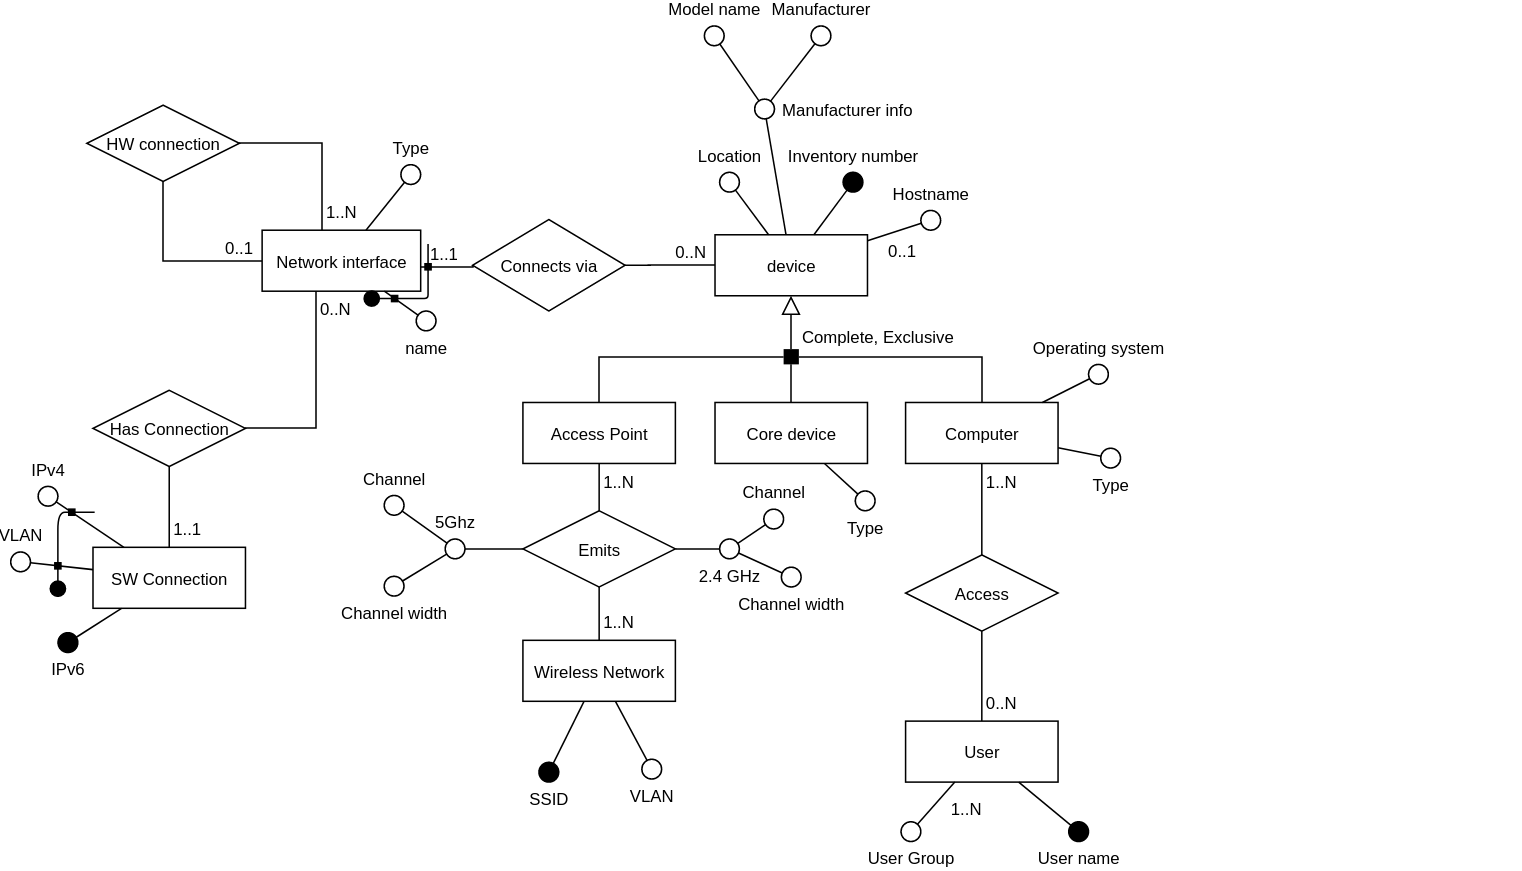
\includegraphics[width=15cm]{er.png}
\caption{ER diagram}
\end{figure}

Device(\underline{invNo}, location, hostname, modelName, manufacturer)

Computer(\underline{device}, os, type)\\
\hspace*{1em}FK: (device) \(\subseteq\) Device(invNo)

User(\underline{username})

UserGroup(\underline{user, name})\\
\hspace*{1em}FK: (user) \(\subseteq\) User(username)

Access(\underline{computer, user})\\
\hspace*{1em}FK: (computer) \(\subseteq\) Computer(device)\\
\hspace*{1em}FK: (user) \(\subseteq\) User(username)

CoreDevice(\underline{device}, type)\\
\hspace*{1em}FK: (device) \(\subseteq\) Device(invNo)

AccessPoint(\underline{device})\\
\hspace*{1em}FK: (device) \(\subseteq\) Device(invNo)

WirelessNet(\underline{ssid}, vlan)

APEmits(\underline{ap, network}, channel5Ghz, width5Ghz, channel2Ghz, width2Ghz)\\
\hspace*{1em}FK: (ap) \(\subseteq\) AccessPoint(device)\\
\hspace*{1em}FK: (network) \(\subseteq\) WirelessNet(ssid)

Interface(\underline{device, name}, type)\\
\hspace*{1em}FK: (device) \(\subseteq\) Device(invNo)

\textit{Source can have multiple targets, but target is connected only to one}\\
source HWConnection(\underline{sourceName, sourceDevice, targetName, targetDevice})\\
\hspace*{1em}FK: (sourceName, sourceDevice) \(\subseteq\) Interface(name, device)\\
\hspace*{1em}FK: (targetName, targetDevice) \(\subseteq\) Interface(name, device)

SWConnection(\underline{ipv6}, \underline{ipv4, vlan}, interface, device)\\
\hspace*{1em}FK: (interface, device) \(\subseteq\) Interface(name, device)


\end{document}
